\documentclass[12pt]{article}
\usepackage{amsfonts,amssymb,amsmath}
\usepackage{graphicx}
%\documentstyle[12pt,amsfonts]{article}
%\documentstyle{article}

\setlength{\topmargin}{-.5in}
\setlength{\oddsidemargin}{0 in}
\setlength{\evensidemargin}{0 in}
\setlength{\textwidth}{6.5truein}
\setlength{\textheight}{8.5truein}
%\input ../basicmath/basicmathmac.tex
%
%\input ../lamacb.tex
\input ../CIS515_Project1/mac.tex
\input ../CIS515_Project1/mathmac.tex

\def\fseq#1#2{(#1_{#2})_{#2\geq 1}}
\def\fsseq#1#2#3{(#1_{#3(#2)})_{#2\geq 1}}
\def\qleq{\sqsubseteq}

%
\begin{document}
\begin{center}
\fbox{{\Large\bf Fall 2016 \hspace*{0.4cm} CIS 515}}\\
\vspace{1cm}
{\Large\bf Fundamentals of Linear Algebra and Optimization\\
Jean Gallier \\
\vspace{0.5cm}
Project 1}\\[10pt]
\end{center}

\noindent {\large Problem 1}\\
\vspace {0.25cm}\noindent
{\bf Adapt N=5 Case} \\

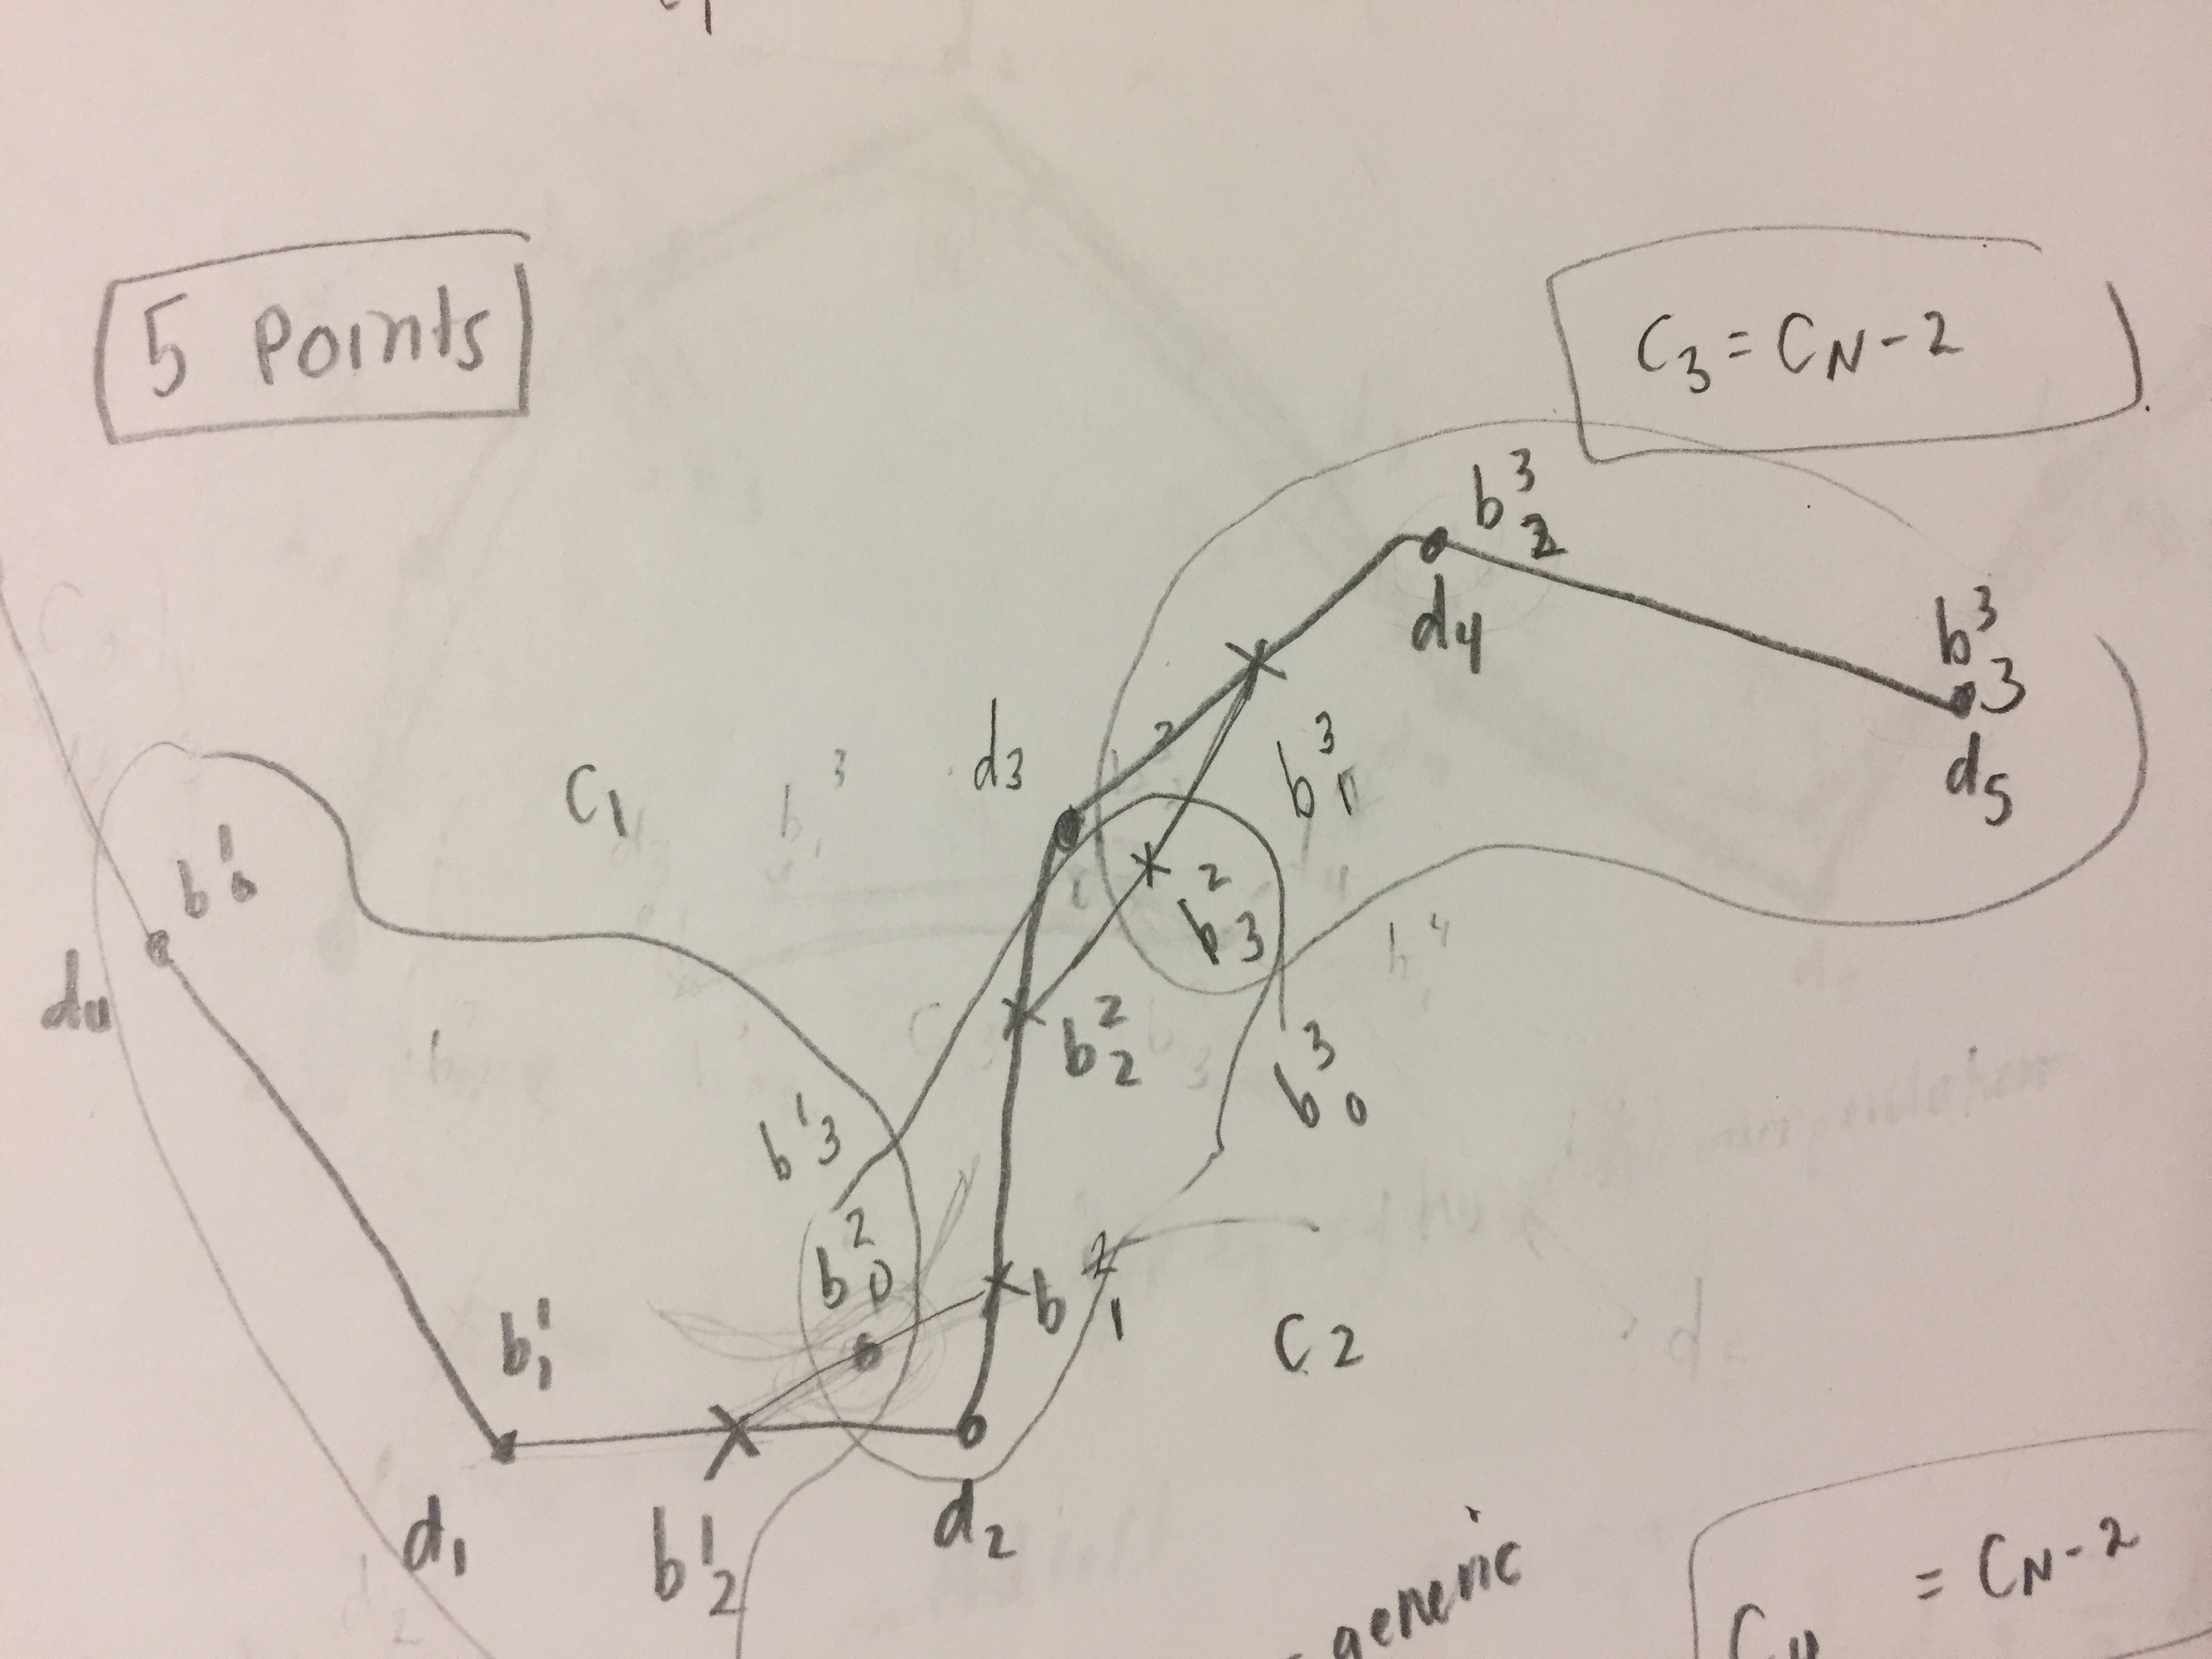
\includegraphics[scale=.1]{5Points}

(C1)
\begin{align*}
b^{1}_{0} =&\; d_0 \\
b^{1}_{1} =&\; d_1 \\
b^{1}_{2} =&\; \frac{1}{2} d_1 + \frac{1}{2}d_2 \\
b^{1}_{3} =&\; \frac{1}{4} b^{1}{2} + \frac{1}{2} b^{2}_{1} =\frac{1}{4}d_1 +\frac{7}{12}d_2 + \frac{1}{6}d_3 \\
\end{align*}

(C2)
\begin{align*}
b^{2}_{0} =&\; \frac{1}{2} b^{1}_{2} + \frac{1}{2} b^{2}_{1}\\
=&\; \frac{1}{4} d_1 + +\frac{7}{12}d_2 + \frac{1}{6}d_3 \\
b^{2}_{1} =&\; \frac{2}{3} d_2 + \frac{1}{3}d_3 \\
b^{2}_{2} =&\; \frac{1}{3} d_2 + \frac{2}{3}d_3 \\
b^{2}_{3} =&\; \frac{1}{2} b^{2}{2} + \frac{1}{2} b^{3}_{1} =\frac{1}{6}d_2 +\frac{4}{6}d_3 + \frac{1}{6}d_4 \\
\end{align*}

(C3)
\begin{align*}
b^{3}_{0} =&\; \frac{1}{2} b^{2}{2} + \frac{1}{2} b^{3}_{1} =\frac{1}{6}d_2 +\frac{4}{6}d_3 + \frac{1}{6}d_4 \\
b^{3}_{1} =&\; \frac{1}{2}d_3 + \frac{1}{2} d_4 \\
b^{3}_{2} =&\; d_4 \\
b^{3}_{3} =&\; d_5 \\
\end{align*}

\vspace {0.25cm}\noindent
{\bf Adapt N=6 Case} \\

\includegraphics[scale=.1]{6Points}

(C1)
\begin{align*}
b^{1}_{0} =&\; d_0 \\
b^{1}_{1} =&\; d_1 \\
b^{1}_{2} =&\; \frac{1}{2} d_1 + \frac{1}{2}d_2 \\
b^{1}_{3} =&\; \frac{1}{4} b^{1}{2} + \frac{1}{2} b^{2}_{1} =\frac{1}{4}d_1 +\frac{7}{12}d_2 + \frac{1}{6}d_3 \\
\end{align*}

(C2)
\begin{align*}
b^{2}_{0} =&\; \frac{1}{2} b^{1}_{2} + \frac{1}{2} b^{2}_{1}\\
=&\; \frac{1}{4} d_1 + +\frac{7}{12}d_2 + \frac{1}{6}d_3 \\
b^{2}_{1} =&\; \frac{2}{3} d_2 + \frac{1}{3}d_3 \\
b^{2}_{2} =&\; \frac{1}{3} d_2 + \frac{2}{3}d_3 \\
b^{2}_{3} =&\; \frac{1}{2} b^{2}{2} + \frac{1}{2} b^{3}_{1} =\frac{1}{6}d_2 +\frac{4}{6}d_3 + \frac{1}{6}d_4 \\
\end{align*}

(C3)
\begin{align*}
b^{3}_{0} =&\; \frac{1}{2} b^{2}{2} + \frac{1}{2} b^{3}_{1} =\frac{1}{6}d_2 +\frac{4}{6}d_3 + \frac{1}{6}d_4 \\
b^{3}_{1} =&\; \frac{2}{3}d_3 + \frac{1}{1} d_4 \\
b^{3}_{2} =&\; \frac{1}{3}d_3 + \frac{2}{3} d_4 \\
b^{3}_{3} =&\; \frac{1}{2} b^{3}_{2} + \frac{1}{2}b^{1}_{4} = \frac{1}{6} d^{3} + \frac{7}{12} d_4 + \frac{1}{4} d_5\\
\end{align*}

(C4)
\begin{align*}
b^{4}_{0} =&\; \frac{1}{2} b^{3}_{2} + \frac{1}{2}b^{1}_{4} = \frac{1}{6} d^{3} + \frac{7}{12} d_4 + \frac{1}{4} d_5\\
b^{4}_{1} =&\; \frac{1}{2}d_4 + \frac{1}{2} d_5 \\
b^{4}_{2} =&\; d_5 \\
b^{4}_{3} =&\; d_6 \\
\end{align*}



\vspace {0.25cm}\noindent
{\bf Adapt N=4 Case Not yet updated} \\

(C1)
\begin{align*}
b^{1}_{0} =&\; d_0 \\
b^{1}_{1} =&\; d_1 \\
b^{1}_{2} =&\; \frac{1}{2} d_1 + \frac{1}{2}d_2 \\
b^{1}_{3} =&\; \frac{1}{4} b^{1}{2} + \frac{1}{2} b^{2}_{1} =\frac{1}{4}d_1 +\frac{7}{12}d_2 + \frac{1}{6}d_3 \\
\end{align*}

(C2)
\begin{align*}
b^{2}_{0} =&\; \frac{1}{2} b^{1}_{2} + \frac{1}{2} b^{2}_{1}\\
=&\; \frac{1}{4} d_1 + +\frac{7}{12}d_2 + \frac{1}{6}d_3 \\
b^{2}_{1} =&\; \frac{2}{3} d_2 + \frac{1}{3}d_3 \\
b^{2}_{2} =&\; \frac{1}{3} d_2 + \frac{2}{3}d_3 \\
b^{2}_{3} =&\; \frac{1}{2} b^{2}{2} + \frac{1}{2} b^{3}_{1} =\frac{1}{6}d_2 +\frac{4}{6}d_3 + \frac{1}{6}d_4 \\
\end{align*}

\noindent {\large Problem 2}\\

\end{document}